\documentclass{article}
\usepackage{german}
\usepackage[latin1]{inputenc}
\usepackage{a4wide}
\usepackage{amssymb}
\usepackage{fancyvrb}
\usepackage{alltt}
\usepackage{epsfig}

\pagestyle{empty}

\begin{document}
\noindent
{\Large \textbf{Exercise}: A Shunting-Problem}
\vspace{0.5cm}


\noindent
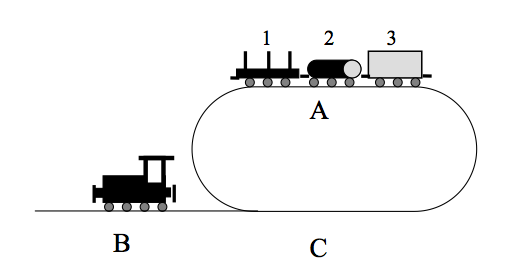
\epsfig{file=rangierProblem, scale=0.8}
\vspace{0.5cm}

\noindent
On the railtrack A there are three wagons that are denoted as wagon 1, 2, and 3.
The locomotive is on the railtrack B.  The goal is to park the wagons in the order 
 3, 1, 2 on the railtrack  C.  Furthermore, the locomotive has to return
to railtrack  B.  The locomotive is able to push or pull any number of wagons.
The locomotive can push and pull wagons simultaneously.

Implement a  \textsc{Setl} program to solve this problem.  In order to do so, the procedure 
 $\texttt{reachable}()$ that has been used so far has to be exchanged for an
 implementation that is more efficient.   A suitable implementation is provided on my 
website.

%Schicken Sie Ihre L�sung bis Montag, den 16.~2.~2008 um 8:00 an meine Email-Adresse:
%\\[0.2cm]
%\hspace*{1.3cm}
%\texttt{stroetmann\symbol{64}ba-stuttgart.de}
%\\[0.2cm]
%Die beste eingehende L�sung wird mit einer Flasche Wein pr�miert.

\end{document}

%%% Local Variables: 
%%% mode: latex
%%% TeX-master: t
%%% End: 
